\documentclass{homework}

\definecolor{bg}{rgb}{0.95,0.95,0.95}

\begin{document}
\frontpage{Þýðendur}{Compiler-NanoMorpho-Bot-up}{Guðmundur Óli Norland}{Egill Ragnarsson}{Snorri Agnarsson}

\begin{question}{Upplýsingar}
\end{question}
\begin{answer}
  \href{https://github.com/slowpokesheep/thydendur/tree/master/nanomorpho_byacc}{Github}
  \begin{description}
    \item[nanomorpho.byaccj] - Er milliþulusmiður og lokaþulusmiður
    \item[nanomorpho.flex] - Er lesgreinir
  \end{description}
  \underline{makefile skipanir}
  \begin{description}
    \item[make] - Býr til alla java og class file'a
    \item[make test] Býr til skrárna \textbf{test.masm}] 
    \item[make gen] Býr til skrárna \textbf{test.mexe}
    \item[make run] - Keyrir \textbf{make test}, \textbf{make gen} og keyrir svo \textbf{test.mexe} skránna
  \end{description}
\end{answer}

\begin{question}{makefile}
\end{question}
\begin{answer}
  \begin{minted}[autogobble,tabsize=2, bgcolor=bg,breaklines,breakanywhere]{makefile}

OUTPUT_DIR=${PWD}/output

PARSER=NanoMorphoParser
TEST_FILE=test
TEST_EXE=${TEST_FILE}.mexe

MORPHO_JAR=../bin/morpho.jar

# Util
printline=$(shell INDEX=0; while [ $${INDEX} -le 80 ]; do printf "-"; INDEX=`expr $$INDEX + 1`; done; printf "\n")

# Colours
blue=\033[0;34m
none=\033[0;m

.PHONY: all main classes flex compiler move clean test

all: main move

main: classes
	@printf "${blue}Making directory <${OUTPUT_DIR}> if it doesn't exist${none}\n"
	if [ ! -d ${OUTPUT_DIR} ]; then mkdir ${OUTPUT_DIR}; fi
	@echo ${printline}

classes: flex
	@printf "${blue}Compiling Lexer, Parser and ParserVal classes${none}\n"
	javac -d output NanoMorphoLexer.java NanoMorphoParser.java NanoMorphoParserVal.java
	@echo ${printline}

flex: compiler
	@printf "${blue}Compiling flex file${none}\n"
	java -jar ../bin/jflex-full-1.7.0.jar nanomorpho.flex
	@echo ${printline}

compiler:
	@printf "${blue}Byacc${none}\n"
	byaccj -Jclass=NanoMorphoParser nanomorpho.byaccj
	@echo ${printline}

move:
	@mv *.java ${OUTPUT_DIR}
	@if [ -f *.java~ ]; then mv *.java~ ${OUTPUT_DIR}; fi

clean:
	rm -rf output

# Testing, generating and running
run: gen # Run .mexe
	@printf "${blue}Running ${TEST_FILE}.mexe${none}\n"
	java -jar ${MORPHO_JAR} ${OUTPUT_DIR}/${TEST_FILE}
	@echo ${printline}
gen: test # Generate .mexe
	@printf "${blue}Compiling ${TEST_FILE}.masm and generating ${TEST_FILE}.mexe${none}\n"
	java -jar ${MORPHO_JAR} -c ${OUTPUT_DIR}/${TEST_FILE}.masm
	@mv ../${TEST_EXE} ${OUTPUT_DIR}/${TEST_EXE}
	@echo ${printline}
test: # Generetae .masm
	@printf "${blue}Testing ${TEST_FILE}.s and generating ${TEST_FILE}.masm${none}\n"
	cd ${OUTPUT_DIR} && java ${PARSER} ../${TEST_FILE}.s
	@mv ${TEST_FILE}.masm ${OUTPUT_DIR}
	@echo ${printline}
  \end{minted}
  \begin{figure}[H]
    \centering
    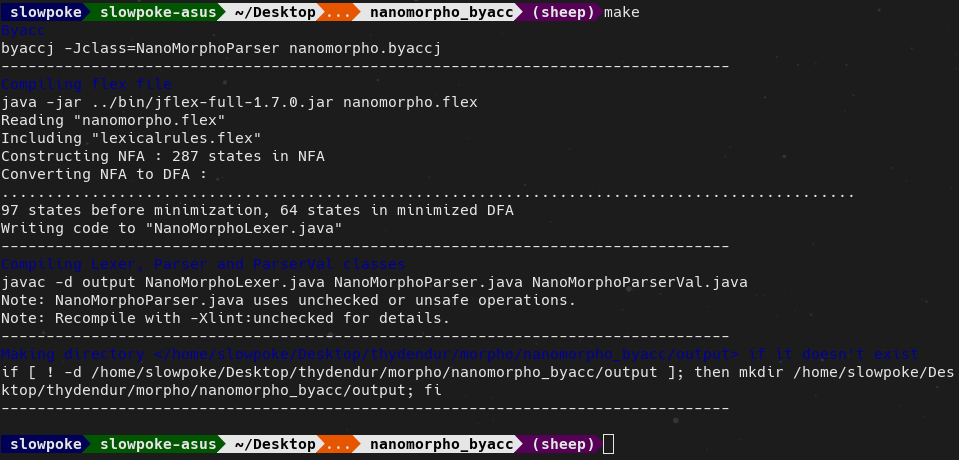
\includegraphics[width=0.8\textwidth]{make.png}
  \end{figure}
\end{answer}

\newpage
\begin{question}{nanomorpho.flex}
\end{question}
\begin{answer}
  \begin{minted}[autogobble,tabsize=2, bgcolor=bg,breaklines,breakanywhere]{java}

import java.io.*;

%%

%public
%class NanoMorphoLexer

%unicode
%byaccj

// Switch these variables on
%line   // yyline
%column // yycolumn
%char   // yychar

%{

// This part becomes a verbatim part of the program text inside
// the class, NanoMorpho.java, that is generated.

public NanoMorphoParser yyparser;

public NanoMorphoLexer(java.io.Reader r, NanoMorphoParser yyparser) {
  this(r);
  this.yyparser = yyparser;
}

// Getters
public int getLine() { return yyline; }
public int getColumn() { return yycolumn; }

%}

/* Regular definitions */

%include lexicalrules.flex

%%

/* Scanning rules */

{_DELIM} {
  yyparser.yylval = new NanoMorphoParserVal(yytext());
  return yycharat(0);
}

{_AND} {
  yyparser.yylval = new NanoMorphoParserVal(yytext());
  return NanoMorphoParser.AND;
}

{_OR} {
  yyparser.yylval = new NanoMorphoParserVal(yytext());
  return NanoMorphoParser.OR;
}

{_STRING} | {_FLOAT} | {_CHAR} | {_INT} | {_BOOL} | null {
  yyparser.yylval = new NanoMorphoParserVal(yytext());
  return NanoMorphoParser.LITERAL;
}

"var" { return NanoMorphoParser.VAR; }
"return" { return NanoMorphoParser.RETURN; }
"while" { return NanoMorphoParser.WHILE; }
"if" { return NanoMorphoParser.IF; }
"elsif" { return NanoMorphoParser.ELSIF; }
"else" { return NanoMorphoParser.ELSE; }

{_NAME} {
  yyparser.yylval = new NanoMorphoParserVal(yytext());
  return NanoMorphoParser.NAME;
}

{_OPNAME} {
  yyparser.yylval = new NanoMorphoParserVal(yytext());
  switch (yytext().charAt(0)) {
    case '^':
    case '?':
    case '~':
        return NanoMorphoParser.OPNAME_1;
    case ':':
        return NanoMorphoParser.OPNAME_2;
    case '|':
        return NanoMorphoParser.OPNAME_3;
    case '&':
        return NanoMorphoParser.OPNAME_4;
    case '!':
    case '=':
    case '<':
    case '>':
        return NanoMorphoParser.OPNAME_5;
    case '+':
    case '-':
        return NanoMorphoParser.OPNAME_6;
    case '*':
    case '/':
    case '%':
        return NanoMorphoParser.OPNAME_7;
    default:
        throw new Error("Invalid opname");
  }
}

// Comment
";;;".*$ { /* Ignore */ }

// White spaces
[ \t\r\n\f] { /* Ignore */ }

// If all rules fail, return an error
[^] {
  return NanoMorphoParser.YYERRCODE;
}
  \end{minted}
\end{answer}

\newpage
\begin{question}{lexicalrules.flex}
\end{question}
\begin{answer}
  \begin{minted}[autogobble,tabsize=2, bgcolor=bg,breaklines,breakanywhere]{java}
    _DIGIT=[0-9]
_FLOAT={_DIGIT}+\.{_DIGIT}+([eE][+-]?{_DIGIT}+)?
_INT={_DIGIT}+
_BOOL=(true|false)
_STRING=\"([^\"\\]|\\b|\\t|\\n|\\f|\\r|\\\"|\\\'|\\\\|(\\[0-3][0-7][0-7])|\\[0-7][0-7]|\\[0-7])*\"
_CHAR=\'([^\'\\]|\\b|\\t|\\n|\\f|\\r|\\\"|\\\'|\\\\|(\\[0-3][0-7][0-7])|(\\[0-7][0-7])|(\\[0-7]))\'
_DELIM=[(){},;=]
_NAME=([:letter:]|\_|{_DIGIT})+
_OPNAME=[\+\-*/!%&=><\:\^\~&|?]+
_AND=&&
_OR=\|\|
  \end{minted}
\end{answer}

\newpage
\begin{question}{nanomorpho.byaccj}
\end{question}
\begin{answer}
  \begin{minted}[autogobble,tabsize=2, bgcolor=bg,breaklines,breakanywhere]{java}
    %{
  import java.io.*;
  import java.util.*;
%}

// Tokens
%token <sval> LITERAL, NAME
%token <sval> OPNAME_1 OPNAME_2 OPNAME_3 OPNAME_4 OPNAME_5 OPNAME_6 OPNAME_7 // Lexer deals with the priority
%token <sval> AND, OR

%token IF, ELSE, ELSIF, WHILE, VAR
%token RETURN, OPNAME

// Args and declarations
%type <ival> funargs
%type <ival> decls decl

// Operators
%type <sval> op

%type <obj> program function
%type <obj> exprs expr binoexpr smallexpr
%type <obj> orexpr andexpr notexpr
%type <obj> ifexpr elsebody
%type <obj> args body

// Precedence and associatives
%right RETURN
%left AND OR

%right '='
%left OPNAME_1 // ~
%right OPNAME_2 // :
%left OPNAME_3 // |
%left OPNAME_4 // &
%left OPNAME_5 // >
%left OPNAME_6 // -
%left OPNAME_7 // %

%left unop

%%

start
  : program { generateProgram(name, ((Vector<Object>)($1)).toArray()); }
  ;

program
  : program function { ((Vector<Object>)($1)).add($2); $$ = $1; } // Multiple functions
  | function { $$ = new Vector<Object>(); ((Vector<Object>)($$)).add($1); } // Single function
  ;

function
  : {
    varCount = 0;
    varTable = new HashMap<String, Integer>();
  }
  NAME '(' funargs ')' '{' decls exprs '}'
  { $$ = new Object[] { $2, $4, varCount, ((Vector<Object>)($8)).toArray() }; }

// Function arguements
funargs
  : { $$ = 0; } // Empty
  | funargs ',' NAME { addVar($3); $$ = $1 + 1; }
  | NAME { addVar($1); $$ = 1; }
  ;

// Declarations
decls
  : { $$ = 0; } // Empty
  | decls decl ';' { $$ = $1 + $2; }
  ;

decl
  : decl ',' NAME { addVar($3); $$ = $1 + 1; }
  | VAR NAME { addVar($2); $$ = 1; }
  ;

// Expressions
exprs
  : exprs expr ';' { ((Vector<Object>)($1)).add($2); $$ = $1; }
  | expr ';' { $$ = new Vector<Object>(); ((Vector<Object>)($$)).add($1); }
  ;

expr
  : RETURN expr { $$ = new Object[] { type.RETURN, $2 }; }
  | NAME '=' expr { $$ = new Object[] { type.STORE, findVar($1), $3 }; }
  | orexpr { $$ = $1; }
  ;

orexpr
  : orexpr OR andexpr { $$ = new Object[] { type.CALL, $2, new Object[] { $1, $3 } }; }
  | andexpr { $$ = $1; }
  ;

andexpr
  : andexpr AND notexpr { $$ = new Object[] { type.CALL, $2, new Object[] { $1, $3 } }; }
  | notexpr { $$ = $1; }
  ;

notexpr
  : '!' notexpr { $$ = new Object[] { type.CALL, '!', new Object[] { $2 } }; }
  | binoexpr { $$ = $1; }
  ;

binoexpr
  : binoexpr OPNAME_1 binoexpr { $$ = new Object[] { type.CALL, $2, new Object[] { $1, $3 } }; } // ~
  | binoexpr OPNAME_2 binoexpr { $$ = new Object[] { type.CALL, $2, new Object[] { $1, $3 } }; } // :
  | binoexpr OPNAME_3 binoexpr { $$ = new Object[] { type.CALL, $2, new Object[] { $1, $3 } }; } // |
  | binoexpr OPNAME_4 binoexpr { $$ = new Object[] { type.CALL, $2, new Object[] { $1, $3 } }; } // &
  | binoexpr OPNAME_5 binoexpr { $$ = new Object[] { type.CALL, $2, new Object[] { $1, $3 } }; } // >
  | binoexpr OPNAME_6 binoexpr { $$ = new Object[] { type.CALL, $2, new Object[] { $1, $3 } }; } // -
  | binoexpr OPNAME_7 smallexpr { $$ = new Object[] { type.CALL, $2, new Object[] { $1, $3 } }; } // %
  | smallexpr { $$ = $1; }
  ;

smallexpr
  : NAME '(' args ')' { $$ = new Object[] { type.CALL, $1, ((Vector<Object>)($3)).toArray() }; }
  | NAME { $$ = new Object[] { type.FETCH, findVar($1) }; }
  | LITERAL { $$ = new Object[] { type.LITERAL, $1 }; }
  | op smallexpr %prec unop { $$ = new Object[] { type.CALL, $1, new Object[] { $2 } }; }
  | '(' expr ')' { $$ = $2; }
  | WHILE '(' expr ')' body { $$ = new Object[] { type.WHILE, $3, new Object[] { type.BODY, $5 } }; }
  | ifexpr { $$ = $1; }
  ;

// If statement
ifexpr
  : IF '(' expr ')' body elsebody { $$ = new Object[] { type.IF, $3, new Object[] { type.BODY, $5 }, $6 }; }
  ;

elsebody
  : { $$ = null; } // Empty
  | ELSIF '(' expr ')' body elsebody { $$ = new Object[] { type.IF, $3, new Object[] { type.BODY, $5 }, $6 }; }
  | ELSE body { $$ = new Object[] { type.IF, new Object[] { type.LITERAL, "true" }, new Object[] { type.BODY, $2 }, null }; }
  ;

// Helpers
args
  : { $$ = new Vector<Object>(); } // Empty
  | args ',' expr { ((Vector<Object>)($1)).add($3); $$ = $1; }
  | expr { $$ = new Vector<Object>(); ((Vector<Object>)($$)).add($1); }
  ;

op
  : OPNAME_1 | OPNAME_2 | OPNAME_3 | OPNAME_4 | OPNAME_5 | OPNAME_6 | OPNAME_7
  ;

body
  : '{' exprs '}' { $$ = ((Vector<Object>)($2)).toArray(); }
  ;

%%

// GENERATE PROGRAM

// The symbol table consists of the following two variables.
private static int varCount;
private static HashMap<String,Integer> varTable;

private NanoMorphoLexer lexer;
private static PrintWriter writer;

private static String name;
private int last_token_read;


// Intermediate code element identification strings
enum type {
  RETURN, STORE, CALL, FETCH, LITERAL, IF, WHILE, BODY
}

// Adds a new variable to the symbol table.
// Throws Error if the variable already exists.
private void addVar(String name) {

  if (varTable.get(name) != null) {
    throw new Error("Variable "+name+" already exists, near line " + lexer.getLine() + 1);
  }
    varTable.put(name,varCount++);
}

// Finds the location of an existing variable.
// Throws Error if the variable does not exist.
private int findVar(String name) {
  Integer res = varTable.get(name);

  if (res == null) {
    throw new Error("Variable "+name+" does not exist, near line " + lexer.getLine() + 1);
  }
    return res;
}

private int yylex() {
  int yyl_return = -1;
  try {
    yylval = null;
    last_token_read = yyl_return = lexer.yylex();

    if (yylval == null ) {
      yylval = new NanoMorphoParserVal(NanoMorphoParser.yyname[yyl_return]);
    }
  }
  catch (IOException e) {
    System.err.println("IO error: " + e);
  }
  return yyl_return;
}

public void yyerror(String error) {
  System.out.println("Error:  " + error);
  System.out.println("Token:  " + NanoMorphoParser.yyname[last_token_read]);
  System.out.printf("Line: %d, Column: %d\n", lexer.getLine(), lexer.getColumn());
  System.exit(1);
}

// Helper

// Returns a new, previously unused, label.
// Useful for control-flow expressions.
private static int nextLabel = 1;

public static int newLabel() {
  return nextLabel++;
}

public void emit(String s) {
  //System.out.println(s);
  writer.println(s);
}

// Final code

public NanoMorphoParser(Reader r) {
  lexer = new NanoMorphoLexer(r, this);
}

public static void main(String args[]) throws IOException {
  NanoMorphoParser yyparser = new NanoMorphoParser(new FileReader(args[0]));
  name = args[0].substring(0, args[0].lastIndexOf('.'));

  writer = new PrintWriter(name + ".masm", "UTF-8");
  yyparser.yyparse();
  writer.close();
}

public void generateProgram(String programname, Object[] funs) {
  emit("\""+programname+".mexe\" = main in");
  emit("!");
  emit("{{");
  
  for (Object f: funs) {
    generateFunction((Object[]) f);
  }

  emit("}}");
  emit("*");
  emit("BASIS;");
}

// [functionName, argCount, varCount, exprs]
public void generateFunction(Object[] fun) {
  String functionName = (String) fun[0];
  int argCount = (Integer) fun[1];
  int varCount = (Integer) fun[2];
  Object[] exprs = (Object[]) fun[3];

  emit("#\"" +functionName+ "[f" +argCount+ "]\" =");
  emit("[");


  for (int i = 0; i < varCount; ++i) {
    emit("(MakeVal null)");
    emit("(Push)");
  }

  for (Object e: exprs) {
    generateExpr((Object[]) e);
  }

  emit("(Return)");
  emit("];");
}

// RETURN, STORE, CALL, FETCH, LITERAL, IF, WHILE, BODY
public void generateExpr(Object[] e) {

  switch((type) e[0]) {
    case RETURN: // ["RETURN", expr]
      generateExpr((Object[]) e[1]);
      emit("(Return)");
      break;
    case STORE: // ["STORE", pos, expr]
      generateExpr((Object[]) e[2]);
      emit("(Store "+e[1]+")");
      break;
    case CALL: // ["CALL", name, args]
      Object[] args = (Object[]) e[2];

      for (Object arg: args) {
        if (args.length == 0) generateExpr((Object[]) arg);
        else generateExprP((Object[]) arg);
      }

      emit("(Call #\""+e[1]+"[f"+args.length+"]\" "+args.length+")");
      break;
    case FETCH: // ["FETCH", pos]
      emit("(Fetch "+e[1]+")");
      break;
    case LITERAL:
      emit("(MakeVal "+e[1]+")");
      break;
    case IF: // ["IF", cond, then, else]
      int labelElse = newLabel();
      int labelEnd = newLabel();

      Object[] ifCond = (Object[]) e[1];
      Object[] ifThen = (Object[]) e[2];

      generateJump(ifCond, 0, labelElse);
      generateExpr(ifThen);

      emit("(Go _"+labelEnd+")");
      emit("_"+labelElse+":");

      Object[] els = (Object[]) e[3];
      if (els != null) {
        generateExpr(els);
      }

      emit("_"+labelEnd+":");
      break;
    case WHILE: // ["WHILE", cond, body]
      int labelStart = newLabel();
      int labelStop = newLabel();

      Object[] whileCond = (Object[]) e[1];
      Object[] whileBody = (Object[]) e[2];

      emit("_"+labelStart+":");

      generateJump(whileCond, 0, labelStop);
      generateBody(whileBody);

      emit("(Go _"+labelStart+")");
      emit("_"+labelStop+":");
      break;
    case BODY: // ["BODY", expr]
      generateBody(e);
      break;
    default:
      throw new Error("Unknown token: " + e[0]);
  }
}

public void generateExprP(Object[] e) {

  switch((type) e[0]) {
    case CALL: // ["CALL", name, args]
      Object[] args = (Object[]) e[2];

      for (Object arg: args) {
        generateExprP((Object[]) arg);
      }

      if (args.length == 0) emit("(Push)");

      emit("(Call #\""+e[1]+"[f"+args.length+"]\" "+args.length+")");
      break;
    case FETCH: // ["FETCH", pos]
      emit("(FetchP "+e[1]+")");
      break;
    case LITERAL: // ["LITERAL", string]
      emit("(MakeValP "+e[1]+")");
      break;
    default:
      throw new Error("Unknown token: " + e[0]);
  }
}

public void generateBody(Object[] e) {
  
  for (Object expr: (Object[]) e[1]) {
    generateExpr((Object[]) expr);
  }
}

public void generateJump(Object[] e, int labelTrue, int labelFalse) {

  switch((type) e[0]) {
    case LITERAL: // ["LITERAL", string]
      String literal = (String) e[1];

      if (literal.equals("false") || literal.equals("null")) {
        if (labelFalse != 0) emit("(Go _"+labelFalse+")");
        return;
      }
      if (labelTrue != 0) emit("(Go _"+labelTrue+")");
      return;
    default:
      generateExprP(e);
      if (labelTrue != 0 ) emit("(GoTrue _"+labelTrue+")");
      if (labelFalse != 0 ) emit("(GoFalse _"+labelFalse+")");
  }
}
  \end{minted}
\end{answer}

\newpage
\begin{question}{test.s}
\end{question}
\begin{answer}
  \begin{minted}[autogobble,tabsize=2, bgcolor=bg,breaklines,breakanywhere]{java}
    ;;; Tests for nanomorpho

;;; Test strings and printing
print_test() {
  var x, y;
  var z;

  y = "Hallo";
  x = "Bye";
  z = "Siggi";

  writeln(x);
  x = "ByeBye";
  writeln(x);

  writeln("Bubbi"++" byggir");
  writeln(x++" "++z);
  printline();
}

;;; Test calculations
calc_test() {
  var x, y, z;
  var result;

  x = 1;
  y = 3;
  z = 5;

  writeln("x = " ++ x ++ " y = " ++ y ++ " z = " ++ z);

  result = 1 + 2 + 3;
  writeln("1 + 2 + 3 = " ++ result);
  
  result = x + y + z;
  writeln("x + y + z = " ++ result);

  result = 4.5 + 3.3 + 6.1;
  writeln("4.5 + 3.3 + 6.1 = " ++ result);

  result = result / 3.1;
  writeln("result / 3.1 = " ++ result);
  printline();
}

;;; Test lists
list_test() {
  var x, y, z, m;
  
  x = 4; y = 3; z = 2;

  write("1:2:3 = "); writeln(1:2:3);
  write("10:20:null = "); writeln(10:20:null);
  writeln("-----");

  writeln("x = " ++ x ++ " y = " ++ y ++ " z = " ++ z);
  writeln("-----");

  write("z:3 = "); writeln(z:3);
  write("x:y:z:3 = "); writeln(x:y:z:3);
  writeln("-----");

  write("head(10:20) = "); writeln(head(10:20));
  write("tail(10:20) = "); writeln(tail(10:20));
  write("tail(z:x):tail(z:y):z = "); writeln(tail(z:x):tail(z:y):z);
  writeln("-----");

  write("\"Bubby\":\"byggir\" = "); writeln("Bubby":"byggir");
  writeln("-----");

  write("Bubbi:null = "); writeln("Bubbi":null);
  printline();
}

;;; Test cond
cond_test(x, y) {

  writeln("x = " ++ x ++ " y = " ++ y);

  if (x) {
    if (y) {
      writeln("x = true y = true");
    }
    else {
      writeln("x = true y = false");
    };
  }
  else {
    if (y) {
      writeln("x = false y = true");
    }
    else {
      writeln("x = false y = false");
    };
  };
  printl();
}

;;; Test more cond
cond2_test(x, y, z) {

  writeln("x = " ++ x ++ " y = " ++ y ++ " z = " ++ z);

  if (x && y && z) {
    writeln("x = true y = true z = true");
  }
  elsif (x || y && z) {
    writeln("x || y && z");
  }
  elsif (x || y && z) {
    writeln("x || y && z");
  }
  elsif (!x && y && !z) {
    writeln("!x && y && !z");
  }
  else {
    writeln("Else");
  };

  printl();
}

;;; Test more cond
cond3_test(x, y, z) {

  writeln("x = " ++ x ++ " y = " ++ y ++ " z = " ++ z);

  if (x == y && x == z) {
    writeln("x == y && x == z");
  }
  elsif (x != z && y == z) {
    writeln("x != z && y == z");
  }
  elsif (x < y) {
    writeln("x < y");
  }
  elsif (x <= y && x != z) {
    writeln("x <= y && x != z");
  }
  elsif (x > y) {
    writeln("x > y");
  }
  elsif (x >= y) {
    writeln("x >= y");
  }
  else {
    writeln("Else");
  };
  printl();
}

;;; Test loops
loop_test() {
  var x;
  x = 0;

  write("while (x < 10) { write(x + \" \") } = ");

  while (x < 10) {
    write(x ++ " ");
    x = x + 1;
  };
  writeln();

  printline();
}

;;; Test non-recursive Fibo
fibo(n) {
  var i, f1, f2, tmp;
  f1 = 1;
  f2 = 1;
  i = 0;

  while (i != n) {
    tmp = f1 + f2;
    f1 = f2;
    f2 = tmp;
    i = i + 1;
  };
  printline();
  f1;
}

;;; Test recursive fibo
f(n) {
  if (n < 2) {
    1;
  }
  else {
    f(n-1) + f(n-2);
  };
}

printline() {
 writeln("-------------------------");
}

printl() {
  writeln("----");
}

main() {
  print_test();
  calc_test();
  list_test();

  cond_test(true, true);
  cond_test(true, false);
  cond_test(false, true);
  cond_test(false, false);

  cond2_test(true, true, true);
  cond2_test(true, false, true);
  cond2_test(false, true, true);
  cond2_test(false, true, false);
  cond2_test(false, false, true);
  printline();

  cond3_test(1, 1, 1); ;;; x == y && x == z
  cond3_test(1, 2, 2); ;;; x != z && y == z

  cond3_test(1, 2, 1); ;;; x < y
  cond3_test(2, 2, 1); ;;; x <= y && x != z

  cond3_test(2, 1, 2); ;;; x > y
  cond3_test(2, 2, 3); ;;; x >= y
  printline();

  loop_test();

	writeln("Not Recursive fibo(35) = " ++ fibo(35));
	writeln("Recursion f(35) = " ++ f(35));
}
  \end{minted}
\end{answer}

\newpage
\begin{question}{test.masm}
\end{question}
\begin{answer}
  \begin{minted}[autogobble,tabsize=2, bgcolor=bg,breaklines,breakanywhere]{java}
    "../test.mexe" = main in
!
{{
#"print_test[f0]" =
[
(MakeVal null)
(Push)
(MakeVal null)
(Push)
(MakeVal null)
(Push)
(MakeVal "Hallo")
(Store 1)
(MakeVal "Bye")
(Store 0)
(MakeVal "Siggi")
(Store 2)
(FetchP 0)
(Call #"writeln[f1]" 1)
(MakeVal "ByeBye")
(Store 0)
(FetchP 0)
(Call #"writeln[f1]" 1)
(MakeValP "Bubbi")
(MakeValP " byggir")
(Call #"++[f2]" 2)
(Call #"writeln[f1]" 1)
(FetchP 0)
(MakeValP " ")
(Call #"++[f2]" 2)
(FetchP 2)
(Call #"++[f2]" 2)
(Call #"writeln[f1]" 1)
(Call #"printline[f0]" 0)
(Return)
];
#"calc_test[f0]" =
[
(MakeVal null)
(Push)
(MakeVal null)
(Push)
(MakeVal null)
(Push)
(MakeVal null)
(Push)
(MakeVal 1)
(Store 0)
(MakeVal 3)
(Store 1)
(MakeVal 5)
(Store 2)
(MakeValP "x = ")
(FetchP 0)
(Call #"++[f2]" 2)
(MakeValP " y = ")
(Call #"++[f2]" 2)
(FetchP 1)
(Call #"++[f2]" 2)
(MakeValP " z = ")
(Call #"++[f2]" 2)
(FetchP 2)
(Call #"++[f2]" 2)
(Call #"writeln[f1]" 1)
(MakeValP 1)
(MakeValP 2)
(Call #"+[f2]" 2)
(MakeValP 3)
(Call #"+[f2]" 2)
(Store 3)
(MakeValP "1 + 2 + 3 = ")
(FetchP 3)
(Call #"++[f2]" 2)
(Call #"writeln[f1]" 1)
(FetchP 0)
(FetchP 1)
(Call #"+[f2]" 2)
(FetchP 2)
(Call #"+[f2]" 2)
(Store 3)
(MakeValP "x + y + z = ")
(FetchP 3)
(Call #"++[f2]" 2)
(Call #"writeln[f1]" 1)
(MakeValP 4.5)
(MakeValP 3.3)
(Call #"+[f2]" 2)
(MakeValP 6.1)
(Call #"+[f2]" 2)
(Store 3)
(MakeValP "4.5 + 3.3 + 6.1 = ")
(FetchP 3)
(Call #"++[f2]" 2)
(Call #"writeln[f1]" 1)
(FetchP 3)
(MakeValP 3.1)
(Call #"/[f2]" 2)
(Store 3)
(MakeValP "result / 3.1 = ")
(FetchP 3)
(Call #"++[f2]" 2)
(Call #"writeln[f1]" 1)
(Call #"printline[f0]" 0)
(Return)
];
#"list_test[f0]" =
[
(MakeVal null)
(Push)
(MakeVal null)
(Push)
(MakeVal null)
(Push)
(MakeVal null)
(Push)
(MakeVal 4)
(Store 0)
(MakeVal 3)
(Store 1)
(MakeVal 2)
(Store 2)
(MakeValP "1:2:3 = ")
(Call #"write[f1]" 1)
(MakeValP 1)
(MakeValP 2)
(MakeValP 3)
(Call #":[f2]" 2)
(Call #":[f2]" 2)
(Call #"writeln[f1]" 1)
(MakeValP "10:20:null = ")
(Call #"write[f1]" 1)
(MakeValP 10)
(MakeValP 20)
(MakeValP null)
(Call #":[f2]" 2)
(Call #":[f2]" 2)
(Call #"writeln[f1]" 1)
(MakeValP "-----")
(Call #"writeln[f1]" 1)
(MakeValP "x = ")
(FetchP 0)
(Call #"++[f2]" 2)
(MakeValP " y = ")
(Call #"++[f2]" 2)
(FetchP 1)
(Call #"++[f2]" 2)
(MakeValP " z = ")
(Call #"++[f2]" 2)
(FetchP 2)
(Call #"++[f2]" 2)
(Call #"writeln[f1]" 1)
(MakeValP "-----")
(Call #"writeln[f1]" 1)
(MakeValP "z:3 = ")
(Call #"write[f1]" 1)
(FetchP 2)
(MakeValP 3)
(Call #":[f2]" 2)
(Call #"writeln[f1]" 1)
(MakeValP "x:y:z:3 = ")
(Call #"write[f1]" 1)
(FetchP 0)
(FetchP 1)
(FetchP 2)
(MakeValP 3)
(Call #":[f2]" 2)
(Call #":[f2]" 2)
(Call #":[f2]" 2)
(Call #"writeln[f1]" 1)
(MakeValP "-----")
(Call #"writeln[f1]" 1)
(MakeValP "head(10:20) = ")
(Call #"write[f1]" 1)
(MakeValP 10)
(MakeValP 20)
(Call #":[f2]" 2)
(Call #"head[f1]" 1)
(Call #"writeln[f1]" 1)
(MakeValP "tail(10:20) = ")
(Call #"write[f1]" 1)
(MakeValP 10)
(MakeValP 20)
(Call #":[f2]" 2)
(Call #"tail[f1]" 1)
(Call #"writeln[f1]" 1)
(MakeValP "tail(z:x):tail(z:y):z = ")
(Call #"write[f1]" 1)
(FetchP 2)
(FetchP 0)
(Call #":[f2]" 2)
(Call #"tail[f1]" 1)
(FetchP 2)
(FetchP 1)
(Call #":[f2]" 2)
(Call #"tail[f1]" 1)
(FetchP 2)
(Call #":[f2]" 2)
(Call #":[f2]" 2)
(Call #"writeln[f1]" 1)
(MakeValP "-----")
(Call #"writeln[f1]" 1)
(MakeValP "\"Bubby\":\"byggir\" = ")
(Call #"write[f1]" 1)
(MakeValP "Bubby")
(MakeValP "byggir")
(Call #":[f2]" 2)
(Call #"writeln[f1]" 1)
(MakeValP "-----")
(Call #"writeln[f1]" 1)
(MakeValP "Bubbi:null = ")
(Call #"write[f1]" 1)
(MakeValP "Bubbi")
(MakeValP null)
(Call #":[f2]" 2)
(Call #"writeln[f1]" 1)
(Call #"printline[f0]" 0)
(Return)
];
#"cond_test[f2]" =
[
(MakeVal null)
(Push)
(MakeVal null)
(Push)
(MakeValP "x = ")
(FetchP 0)
(Call #"++[f2]" 2)
(MakeValP " y = ")
(Call #"++[f2]" 2)
(FetchP 1)
(Call #"++[f2]" 2)
(Call #"writeln[f1]" 1)
(FetchP 0)
(GoFalse _1)
(FetchP 1)
(GoFalse _3)
(MakeValP "x = true y = true")
(Call #"writeln[f1]" 1)
(Go _4)
_3:
(MakeValP "x = true y = false")
(Call #"writeln[f1]" 1)
(Go _6)
_5:
_6:
_4:
(Go _2)
_1:
(FetchP 1)
(GoFalse _9)
(MakeValP "x = false y = true")
(Call #"writeln[f1]" 1)
(Go _10)
_9:
(MakeValP "x = false y = false")
(Call #"writeln[f1]" 1)
(Go _12)
_11:
_12:
_10:
(Go _8)
_7:
_8:
_2:
(Call #"printl[f0]" 0)
(Return)
];
#"cond2_test[f3]" =
[
(MakeVal null)
(Push)
(MakeVal null)
(Push)
(MakeVal null)
(Push)
(MakeValP "x = ")
(FetchP 0)
(Call #"++[f2]" 2)
(MakeValP " y = ")
(Call #"++[f2]" 2)
(FetchP 1)
(Call #"++[f2]" 2)
(MakeValP " z = ")
(Call #"++[f2]" 2)
(FetchP 2)
(Call #"++[f2]" 2)
(Call #"writeln[f1]" 1)
(FetchP 0)
(FetchP 1)
(Call #"&&[f2]" 2)
(FetchP 2)
(Call #"&&[f2]" 2)
(GoFalse _13)
(MakeValP "x = true y = true z = true")
(Call #"writeln[f1]" 1)
(Go _14)
_13:
(FetchP 0)
(FetchP 1)
(FetchP 2)
(Call #"&&[f2]" 2)
(Call #"||[f2]" 2)
(GoFalse _15)
(MakeValP "x || y && z")
(Call #"writeln[f1]" 1)
(Go _16)
_15:
(FetchP 0)
(FetchP 1)
(FetchP 2)
(Call #"&&[f2]" 2)
(Call #"||[f2]" 2)
(GoFalse _17)
(MakeValP "x || y && z")
(Call #"writeln[f1]" 1)
(Go _18)
_17:
(FetchP 0)
(Call #"![f1]" 1)
(FetchP 1)
(Call #"&&[f2]" 2)
(FetchP 2)
(Call #"![f1]" 1)
(Call #"&&[f2]" 2)
(GoFalse _19)
(MakeValP "!x && y && !z")
(Call #"writeln[f1]" 1)
(Go _20)
_19:
(MakeValP "Else")
(Call #"writeln[f1]" 1)
(Go _22)
_21:
_22:
_20:
_18:
_16:
_14:
(Call #"printl[f0]" 0)
(Return)
];
#"cond3_test[f3]" =
[
(MakeVal null)
(Push)
(MakeVal null)
(Push)
(MakeVal null)
(Push)
(MakeValP "x = ")
(FetchP 0)
(Call #"++[f2]" 2)
(MakeValP " y = ")
(Call #"++[f2]" 2)
(FetchP 1)
(Call #"++[f2]" 2)
(MakeValP " z = ")
(Call #"++[f2]" 2)
(FetchP 2)
(Call #"++[f2]" 2)
(Call #"writeln[f1]" 1)
(FetchP 0)
(FetchP 1)
(Call #"==[f2]" 2)
(FetchP 0)
(FetchP 2)
(Call #"==[f2]" 2)
(Call #"&&[f2]" 2)
(GoFalse _23)
(MakeValP "x == y && x == z")
(Call #"writeln[f1]" 1)
(Go _24)
_23:
(FetchP 0)
(FetchP 2)
(Call #"!=[f2]" 2)
(FetchP 1)
(FetchP 2)
(Call #"==[f2]" 2)
(Call #"&&[f2]" 2)
(GoFalse _25)
(MakeValP "x != z && y == z")
(Call #"writeln[f1]" 1)
(Go _26)
_25:
(FetchP 0)
(FetchP 1)
(Call #"<[f2]" 2)
(GoFalse _27)
(MakeValP "x < y")
(Call #"writeln[f1]" 1)
(Go _28)
_27:
(FetchP 0)
(FetchP 1)
(Call #"<=[f2]" 2)
(FetchP 0)
(FetchP 2)
(Call #"!=[f2]" 2)
(Call #"&&[f2]" 2)
(GoFalse _29)
(MakeValP "x <= y && x != z")
(Call #"writeln[f1]" 1)
(Go _30)
_29:
(FetchP 0)
(FetchP 1)
(Call #">[f2]" 2)
(GoFalse _31)
(MakeValP "x > y")
(Call #"writeln[f1]" 1)
(Go _32)
_31:
(FetchP 0)
(FetchP 1)
(Call #">=[f2]" 2)
(GoFalse _33)
(MakeValP "x >= y")
(Call #"writeln[f1]" 1)
(Go _34)
_33:
(MakeValP "Else")
(Call #"writeln[f1]" 1)
(Go _36)
_35:
_36:
_34:
_32:
_30:
_28:
_26:
_24:
(Call #"printl[f0]" 0)
(Return)
];
#"loop_test[f0]" =
[
(MakeVal null)
(Push)
(MakeVal 0)
(Store 0)
(MakeValP "while (x < 10) { write(x + \" \") } = ")
(Call #"write[f1]" 1)
_37:
(FetchP 0)
(MakeValP 10)
(Call #"<[f2]" 2)
(GoFalse _38)
(FetchP 0)
(MakeValP " ")
(Call #"++[f2]" 2)
(Call #"write[f1]" 1)
(FetchP 0)
(MakeValP 1)
(Call #"+[f2]" 2)
(Store 0)
(Go _37)
_38:
(Call #"writeln[f0]" 0)
(Call #"printline[f0]" 0)
(Return)
];
#"fibo[f1]" =
[
(MakeVal null)
(Push)
(MakeVal null)
(Push)
(MakeVal null)
(Push)
(MakeVal null)
(Push)
(MakeVal null)
(Push)
(MakeVal 1)
(Store 2)
(MakeVal 1)
(Store 3)
(MakeVal 0)
(Store 1)
_39:
(FetchP 1)
(FetchP 0)
(Call #"!=[f2]" 2)
(GoFalse _40)
(FetchP 2)
(FetchP 3)
(Call #"+[f2]" 2)
(Store 4)
(Fetch 3)
(Store 2)
(Fetch 4)
(Store 3)
(FetchP 1)
(MakeValP 1)
(Call #"+[f2]" 2)
(Store 1)
(Go _39)
_40:
(Call #"printline[f0]" 0)
(Fetch 2)
(Return)
];
#"f[f1]" =
[
(MakeVal null)
(Push)
(FetchP 0)
(MakeValP 2)
(Call #"<[f2]" 2)
(GoFalse _41)
(MakeVal 1)
(Go _42)
_41:
(FetchP 0)
(MakeValP 1)
(Call #"-[f2]" 2)
(Call #"f[f1]" 1)
(FetchP 0)
(MakeValP 2)
(Call #"-[f2]" 2)
(Call #"f[f1]" 1)
(Call #"+[f2]" 2)
(Go _44)
_43:
_44:
_42:
(Return)
];
#"printline[f0]" =
[
(MakeValP "-------------------------")
(Call #"writeln[f1]" 1)
(Return)
];
#"printl[f0]" =
[
(MakeValP "----")
(Call #"writeln[f1]" 1)
(Return)
];
#"main[f0]" =
[
(Call #"print_test[f0]" 0)
(Call #"calc_test[f0]" 0)
(Call #"list_test[f0]" 0)
(MakeValP true)
(MakeValP true)
(Call #"cond_test[f2]" 2)
(MakeValP true)
(MakeValP false)
(Call #"cond_test[f2]" 2)
(MakeValP false)
(MakeValP true)
(Call #"cond_test[f2]" 2)
(MakeValP false)
(MakeValP false)
(Call #"cond_test[f2]" 2)
(MakeValP true)
(MakeValP true)
(MakeValP true)
(Call #"cond2_test[f3]" 3)
(MakeValP true)
(MakeValP false)
(MakeValP true)
(Call #"cond2_test[f3]" 3)
(MakeValP false)
(MakeValP true)
(MakeValP true)
(Call #"cond2_test[f3]" 3)
(MakeValP false)
(MakeValP true)
(MakeValP false)
(Call #"cond2_test[f3]" 3)
(MakeValP false)
(MakeValP false)
(MakeValP true)
(Call #"cond2_test[f3]" 3)
(Call #"printline[f0]" 0)
(MakeValP 1)
(MakeValP 1)
(MakeValP 1)
(Call #"cond3_test[f3]" 3)
(MakeValP 1)
(MakeValP 2)
(MakeValP 2)
(Call #"cond3_test[f3]" 3)
(MakeValP 1)
(MakeValP 2)
(MakeValP 1)
(Call #"cond3_test[f3]" 3)
(MakeValP 2)
(MakeValP 2)
(MakeValP 1)
(Call #"cond3_test[f3]" 3)
(MakeValP 2)
(MakeValP 1)
(MakeValP 2)
(Call #"cond3_test[f3]" 3)
(MakeValP 2)
(MakeValP 2)
(MakeValP 3)
(Call #"cond3_test[f3]" 3)
(Call #"printline[f0]" 0)
(Call #"loop_test[f0]" 0)
(MakeValP "Not Recursive fibo(35) = ")
(MakeValP 35)
(Call #"fibo[f1]" 1)
(Call #"++[f2]" 2)
(Call #"writeln[f1]" 1)
(MakeValP "Recursion f(35) = ")
(MakeValP 35)
(Call #"f[f1]" 1)
(Call #"++[f2]" 2)
(Call #"writeln[f1]" 1)
(Return)
];
}}
*
BASIS;
  \end{minted}
  \begin{figure}[H]
    \centering
    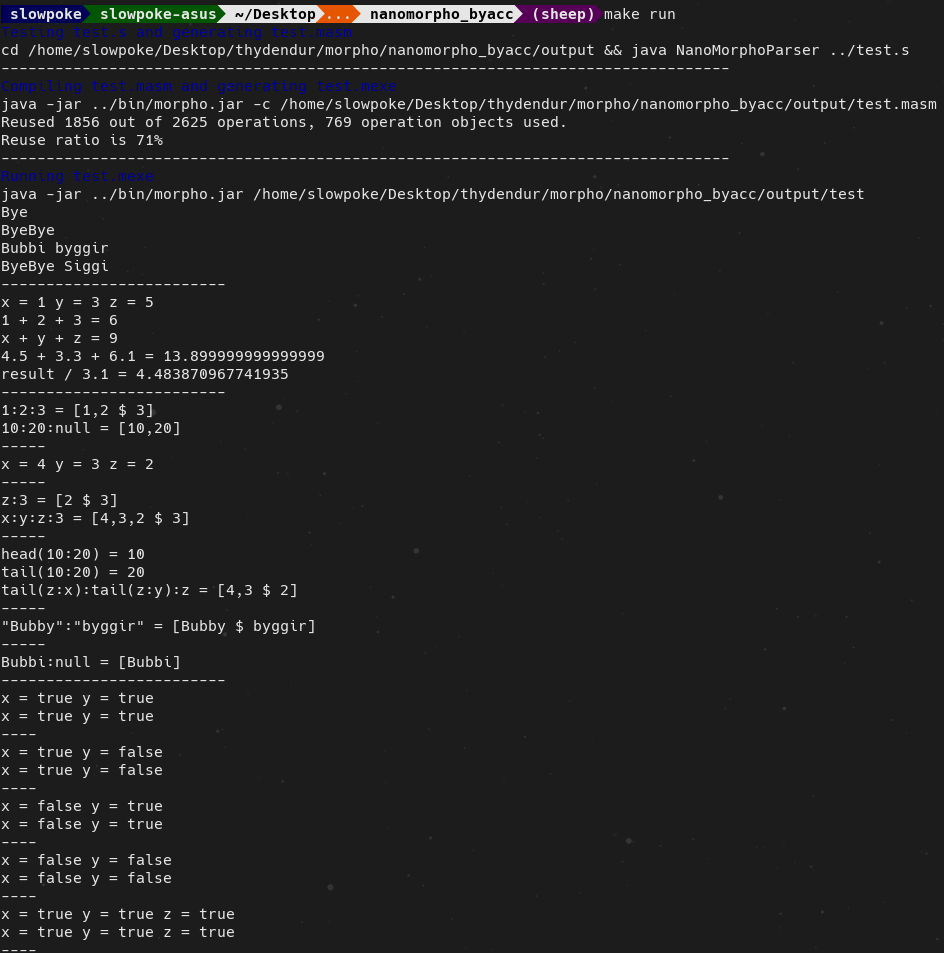
\includegraphics[width=0.8\textwidth]{test_s1.png}
  \end{figure}
  \begin{figure}[H]
    \centering
    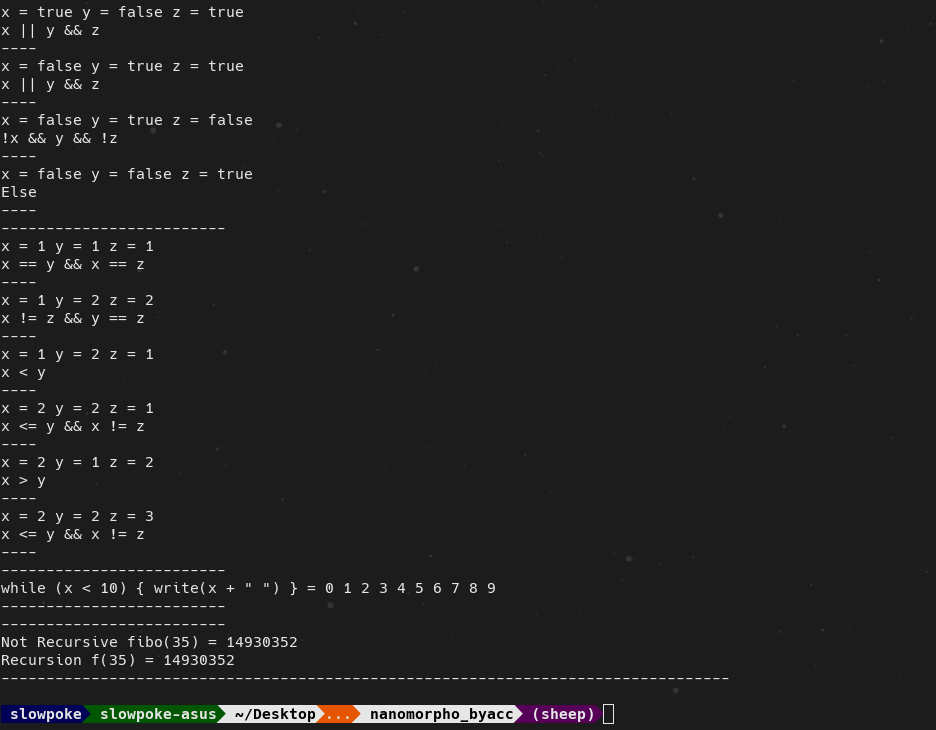
\includegraphics[width=0.8\textwidth]{test_s2.png}
  \end{figure}
\end{answer}

\end{document}
